% Figure 1 (architecture): two-split framework, compiled standalone; the 300 dpi PNG is made with pdftoppm.
% Split 1 = vision and semantic perception (StrongDINOv2Seg + OpenCV morphological / watershed footprint extraction); Split 2 = geospatial cost surface and shared-network routing.
% Parameters are those of the code: scripts/run_tiled_inference.py (tile 560, stride 420, margin 70), scripts/extract_buildings_v8.py (neck ratio 0.65),
% scripts/audit_facilities.py (snap 35 m), src/multivillage/clearance.py (5 m grid, 3.6 m clearance), scripts/plan_network_v2.py (K=3, greedy weight / marginal cost).
\documentclass[tikz,border=3pt]{standalone}
\usetikzlibrary{arrows.meta,calc}
\usepackage{amsmath}
\usepackage{helvet}
\renewcommand{\familydefault}{\sfdefault}
\definecolor{tG}{HTML}{F2F3F5}  % neutral grey: data in / out
\definecolor{tB}{HTML}{E5EBF2}  % muted blue: Split 1 (learning and extraction)
\definecolor{tA}{HTML}{F5EEDD}  % muted amber: Split 2 (routing)
\hyphenpenalty=10000 \exhyphenpenalty=10000
\begin{document}
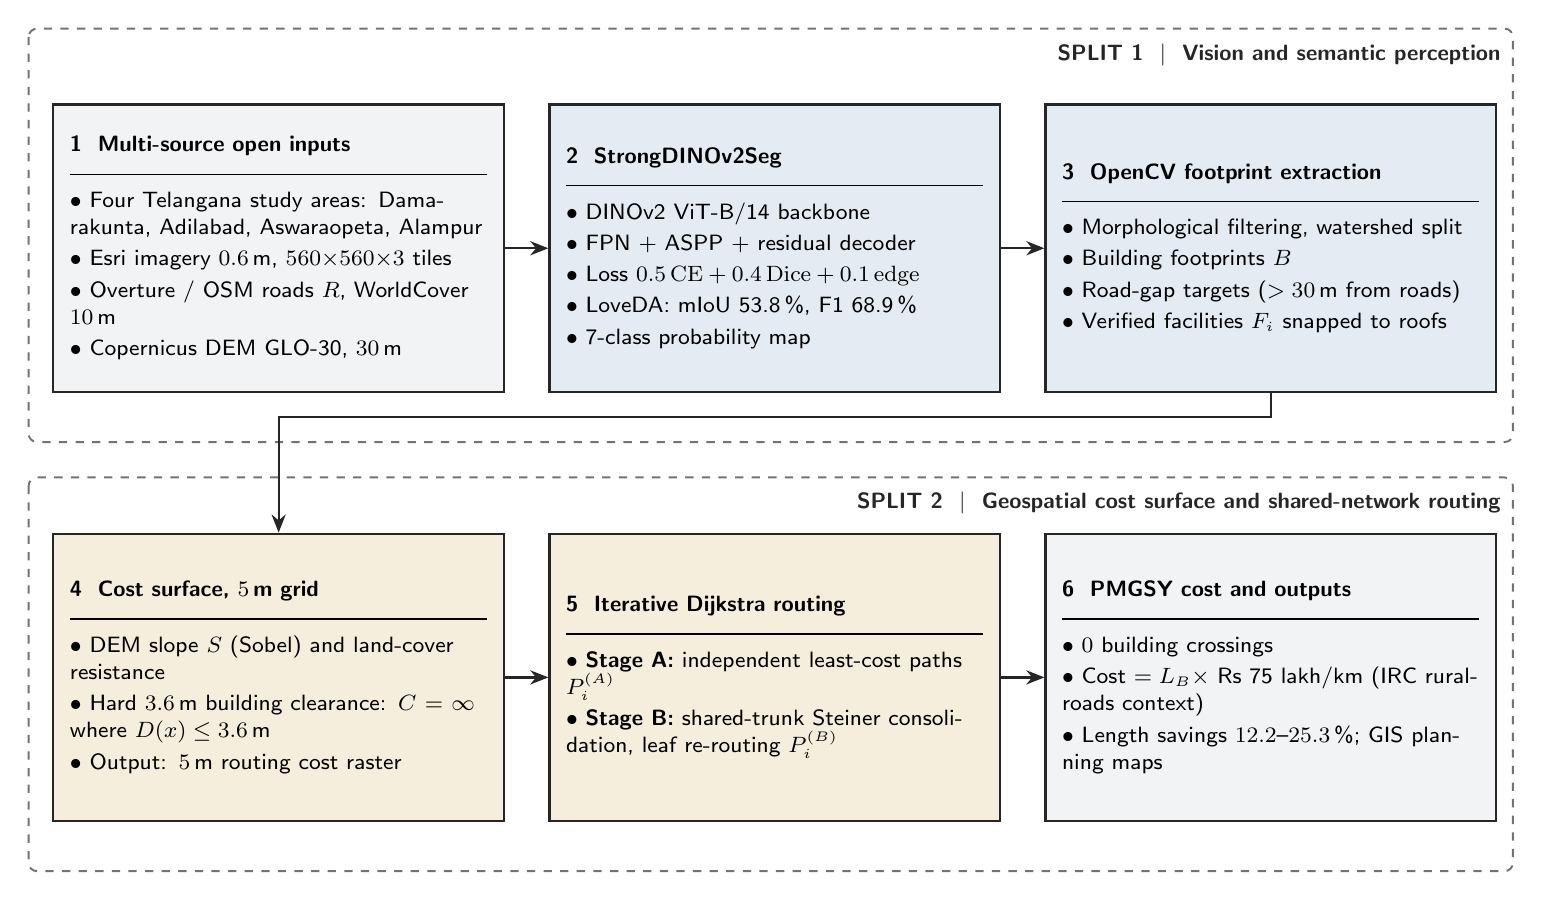
\begin{tikzpicture}[x=1cm,y=1cm]
\tikzset{
  blk/.style={draw=black!85,line width=0.8pt,fill=#1,text width=5.3cm,inner xsep=6pt,inner ysep=5pt,align=left,anchor=north west,minimum height=3.65cm,font=\fontsize{7.8}{9.8}\selectfont},
  arr/.style={-{Stealth[length=2.3mm,width=1.8mm]},line width=0.8pt,black!85},
  frame/.style={draw=black!55,dashed,line width=0.7pt,rounded corners=3pt},
  tag/.style={anchor=east,font=\fontsize{8.4}{10}\selectfont\bfseries,text=black!85,inner sep=0pt}
}
\newcommand{\hd}[2]{\textbf{#1\ \ #2}\\[-1.5pt]\rule{5.3cm}{0.5pt}\\[2pt]}
\newcommand{\li}[1]{$\bullet$\ #1\\[1.5pt]}
% ---- Split 1
\draw[frame] (-0.3,0.95) rectangle (18.55,-4.3);
\node[tag] at (18.4,0.62) {SPLIT 1\ \ $\vert$\ \ Vision and semantic perception};
\node[blk=tG] at (0,0) (s1) {\hd{1}{Multi-source open inputs}
  \li{Four Telangana study areas: Damarakunta, Adilabad, Aswaraopeta, Alampur}
  \li{Esri imagery $0.6$\,m, $560{\times}560{\times}3$ tiles}
  \li{Overture / OSM roads $R$, WorldCover $10$\,m}
  \li{Copernicus DEM GLO-30, $30$\,m}};
\node[blk=tB] at (6.3,0) (s2) {\hd{2}{StrongDINOv2Seg}
  \li{DINOv2 ViT-B/14 backbone}
  \li{FPN $+$ ASPP $+$ residual decoder}
  \li{Loss $0.5\,\mathrm{CE}+0.4\,\mathrm{Dice}+0.1\,\mathrm{edge}$}
  \li{LoveDA: mIoU 53.8\,\%, F1 68.9\,\%}
  \li{7-class probability map}};
\node[blk=tB] at (12.6,0) (s3) {\hd{3}{OpenCV footprint extraction}
  \li{Morphological filtering, watershed split}
  \li{Building footprints $B$}
  \li{Road-gap targets ($>30$\,m from roads)}
  \li{Verified facilities $F_i$ snapped to roofs}};
% ---- Split 2
\draw[frame] (-0.3,-4.75) rectangle (18.55,-9.75);
\node[tag] at (18.4,-5.08) {SPLIT 2\ \ $\vert$\ \ Geospatial cost surface and shared-network routing};
\node[blk=tA] at (0,-5.45) (s4) {\hd{4}{Cost surface, $5$\,m grid}
  \li{DEM slope $S$ (Sobel) and land-cover resistance}
  \li{Hard $3.6$\,m building clearance: $C=\infty$ where $D(x)\le3.6$\,m}
  \li{Output: $5$\,m routing cost raster}};
\node[blk=tA] at (6.3,-5.45) (s5) {\hd{5}{Iterative Dijkstra routing}
  \li{\textbf{Stage A:} independent least-cost paths $P_i^{(A)}$}
  \li{\textbf{Stage B:} shared-trunk Steiner consolidation, leaf re-routing $P_i^{(B)}$}};
\node[blk=tG] at (12.6,-5.45) (s6) {\hd{6}{PMGSY cost and outputs}
  \li{$0$ building crossings}
  \li{Cost $=L_B\times$ Rs 75 lakh/km (IRC rural-roads context)}
  \li{Length savings $12.2$--$25.3$\,\%; GIS planning maps}};
% ---- arrows
\draw[arr] (s1.east) -- (s2.west);
\draw[arr] (s2.east) -- (s3.west);
\draw[arr] (s3.south) -- ++(0,-0.3) -| (s4.north);
\draw[arr] (s4.east) -- (s5.west);
\draw[arr] (s5.east) -- (s6.west);
\end{tikzpicture}
\end{document}
